%; whizzy paragraph -pdf xpdf -latex ./whizzypdfptex.sh
%; whizzy-paragraph "^\\\\begin{frame}\\|\\\\emtext"
% latex beamer presentation.
% platex, latex-beamer でコンパイルすることを想定。 

%     Tokyo Debian Meeting resources
%     Copyright (C) 2012 Junichi Uekawa
%     Copyright (C) 2011 Nobuhiro Iwamatsu

%     This program is free software; you can redistribute it and/or modify
%     it under the terms of the GNU General Public License as published by
%     the Free Software Foundation; either version 2 of the License, or
%     (at your option) any later version.

%     This program is distributed in the hope that it will be useful,
%     but WITHOUT ANY WARRANTY; without even the implied warreanty of
%     MERCHANTABILITY or FITNESS FOR A PARTICULAR PURPOSE.  See the
%     GNU General Public License for more details.

%     You should have received a copy of the GNU General Public License
%     along with this program; if not, write to the Free Software
%     Foundation, Inc., 51 Franklin St, Fifth Floor, Boston, MA  02110-1301 USA

\documentclass[cjk,dvipdfmx,12pt]{beamer}
\usetheme{Tokyo}
\usepackage{monthlypresentation}

%  preview (shell-command (concat "evince " (replace-regexp-in-string "tex$" "pdf"(buffer-file-name)) "&")) 
%  presentation (shell-command (concat "xpdf -fullscreen " (replace-regexp-in-string "tex$" "pdf"(buffer-file-name)) "&"))
%  presentation (shell-command (concat "evince " (replace-regexp-in-string "tex$" "pdf"(buffer-file-name)) "&"))

%http://www.naney.org/diki/dk/hyperref.html
%日本語EUC系環境の時
\AtBeginDvi{\special{pdf:tounicode EUC-UCS2}}
%シフトJIS系環境の時
%\AtBeginDvi{\special{pdf:tounicode 90ms-RKSJ-UCS2}}

\title{東京エリアDebian勉強会}
\subtitle{第85回 2012年2月度}
\author{野島 貴英\\nozzy@debian.or.jp}
\date{2012年2月18日}
\logo{
\includegraphics[width=8cm]{image200607/openlogo-light.eps}}

\begin{document}

\frame{\titlepage{}}

\begin{frame}{設営準備にご協力ください。}
会場設営などよろしくおねがいします。
\end{frame}

\section{Agenda}
\begin{frame}{Agenda}
\begin{minipage}[t]{0.45\hsize}
  \begin{itemize}
  \item 注意事項
	\begin{itemize}
	 \item 飲食禁止
	 \item 宗教禁止
	 \item 営利活動禁止
	\end{itemize}
   \item 最近あったDebian関連のイベント報告
	\begin{itemize}
        \item 第84回 東京エリアDebian勉強会
	\end{itemize}
 \end{itemize}
\end{minipage} 
\begin{minipage}[t]{0.45\hsize}
 \begin{itemize}
   \item 事前課題紹介
   \item Debian Trivia Quiz
   \item Debian開発者の為のKDE環境あれこれ
   \item 月刊デブヘルパー 第4回
   \item cmake使ってみた
  \end{itemize}
\end{minipage}
\end{frame}

\section{イベント報告}
\emtext{イベント報告}
\emtext{第84回東京エリアDebian勉強会}

\begin{frame}{第84回東京エリアDebian勉強会}
\begin{itemize}
\item 開催場所は あんさんぶる荻窪
\item WEBシステムを意識した発表が多かったです(脆弱性、VPS、twitter連携)
\item 今年の勉強会テーマはいろいろアイデアがあって刺激的でした。
\item 新年会もやりましたよ!
\end{itemize}
\end{frame}

\section{事前課題}
\emtext{事前課題}
{\footnotesize
 \begin{prework}{ 鈴木崇文 }

gnomeでdesktopを利用しています。
工夫というほどではないですが、便利なツールとしてKDE系のアプリやEBViewを使っています。
リモートデスクトップ(RDP) & VNC 用には、KRDC を使い、スクリーンショット用には KSnapshot を使っています。
あとは英辞郎を購入して、EBViewでいつでも翻訳できるようにしています。
\end{prework}

\begin{prework}{ dictoss(杉本 典充) }

低性能マシンはstartx+icewm、中高性能マシンはgdm+xfce4かgnomeと使い分けています。KDEは最近使ってないです。(KDEは重そうなイメージがある)
カスタマイズしているのは、ページャの個数を6つに増やしている、複数のターミナルを重ならないように同時起動するシェルスクリプトを作り一発で画面をターミナルで埋め尽くせるようにしています。(昔タイル型ウィンドウマネージャ使えばいいのに、とか突っ込まれました)
\end{prework}

\begin{prework}{ yamamoto }

メインに使っているのは、録画サーバも兼ねた Debian squeeze (amd64) です。
外出時は気分次第で、sid の i386 ネットブックと sid の amd64 ノート PC を選んでいます。
どれも、特に何の変てつもない、ただの KDE 環境です。

デスクトップとしての見た目は、壁紙すらデフォルトのままで、改造してませんが、機体としては家の LAN にぶら下がったマシン間を「何か(?)」が行き来する、魔改造スクリプトがいくつか仕込んであり、ものぐさな私にはとっても快適です。
\end{prework}

\begin{prework}{ 野島 貴英 }

GNOME 3.2.2をDebianで利用しています。unstableではもの足りず、experimentalからupgradeして引っ張ってきてます。特にクールなカスタマイズは何もしてないですが、gnome-shellがjavascriptなど解釈できるということから、将来ちょっとしたガジェットぐらい作ってみたいなーと思うこの頃です。あと、gxconsole( \url{http://gnomefiles.org/content/show.php/gxconsole?content=132145} )がGNOME3.2.2になっても、やっぱり欲しかったので、GNOME 3.2.2用に移植したい...
\end{prework}

\begin{prework}{ 日比野 啓 }

普段はタイル型ウィンドウマネージャの XMonad を使っています。
マルチディスプレイに対するサポートが使いやすくてプレゼンのときにも便利で気にいっています。
最近、趣味のプログラミングのメインで使っている言語が Haskell なので、
Haskellでカスタマイズできることも魅力です。
gnome-session との組合せも使ってみましたが、なぜか sid ではうまく動かなくて残念。
あと、画面の上下が狭くなるのが嫌なので、なんとかする方法が知りたい。

\end{prework}

}

\section{DWN quiz}
\emtext{DWN quiz}
\begin{frame}{Debian 常識クイズ}

Debian の常識、もちろん知ってますよね?
知らないなんて恥ずかしくて、知らないとは言えないあんなことやこんなこと、
みんなで確認してみましょう。

今回の出題範囲は\url{debian-devel-announce@lists.debian.org},
\url{debian-devel@lists.debian.org} に投稿された
内容とDebian Project Newsなどからです。

\end{frame}

\subsection{問題}
%; whizzy-master ../debianmeetingresume201201.tex
% $B0J>e$N@_Dj$r$7$F$$$k$?$a!"$3$N%U%!%$%k$G(B M-x whizzytex $B$9$k$H!"(Bwhizzytex$B$,MxMQ$G$-$^$9!#(B
%

\santaku
{2/14$B:"$K(Bwheezy$B$K4X$7$F8xJg$,9T$o$l$^$7$?!#2?$N8xJg$G$7$g$&$+!)(B}
{I18N$B4X78$N%5!<%P!<%7%9%F%`:F9=C[$N8xJg(B}
{$B1~1gCDD9(B/$B%$%a!<%8%?%l%s%H$N8xJg(B}
{Look and Feel$B$N%"!<%HJ,Ln$K4X$9$k8xJg(B}
{C}
{$BH~=Q(B/$B%^%s%,(B/$B%$%i%9%H$KOS$N3P$($,$"$k?M$O$<$R!#@$3&E*$KM-L>$K$J$l$k$+$b$7$l$^$;$s!#(B\url{http://wiki.debian.org/DebianDesktop/Artwork/Wheezy}}

\santaku
{$B:#G/(B2$B7n$K%;%-%e%j%F%#%"%C%W%G!<%H$,=*N;$7$?(BDebian$B$N%P!<%8%g%s$O2?$G$7$g$&(B?}
{lenny}
{sarge}
{woody}
{A}
{Debian$B4X78<T$K$O>o<1$G$7$?$M!#(B}

\santaku
{1/25$B$K(Balioth$B$K$J$K$,$*$-$?$+(B}
{vasks.debian.org$B$,5/F0$7$J$/$J$C$?(B}
{wagner.debian.org$B$,5/F0$7$J$/$J$C$?(B}
{churro$B$,5/F0$7$J$/$J$C$?(B}
{A}
{$BEE8;$bF~$i$J$+$C$?$=$&$G$9!#(Balioth$B$H$O4X78$J$$$G$9$,!"(Bchurro$B!J(Bi18n$B%a%s%F4X78<T$i$N@.2LJ*F~$l$?%5!<%P!<!K$bD4;R0-$+$C$?$G$9!#(B}

\santaku
{$B:#G/$N(BDebConf12$B$O$$$D3+$+$l$kM=Dj(B?}
{2012/7/1-7/7}
{2012/7/8-7/14}
{2012/$B$N$*K_(B}
{B}
{$B$=$m$=$m(Bsuponcerd$B$J;22C<TJg=8F08~$r%A%'%C%/$7$?J}$,$h$$$+$b$7$l$^$;$s(B}

\santaku
{wheezy$B$KF~$kM=Dj$N(BLinux$B%+!<%M%k%P!<%8%g%s$O$$$/$D$G$7$g$&!)(B}
{3.0$B7ONs(B}
{3.1$B7ONs(B}
{3.2$B7ONs(B}
{C}
{$B$+$J$j:G?7$G$9$M!#%I%i%$%P3+H/$r4hD%$j$^$7$g$&!#(B}

\santaku
{$B%$%s%9%H!<%k(B/$B%"%C%W%0%l!<%I(B/$B>C5n%F%9%H$rC4$&(BQA$B%A!<%`$N6/NO$J%D!<%k$NL>A0$O!)(B}
{init}
{piuparts}
{upstart}
{B}
{Package Install, UPgrading And Removal Testing Sute$B$NN,$@$=$&$G$9!#(B}

\santaku
{2/18$B:G?7$N(BDebian$B$N0BDjHG$N%j%j!<%9HV9f$O$$$/$D$G$7$g$&$+!)(B}
{6.0.1}
{6.0.2}
{6.0.4}
{C}
{$B$3$NA0%"%J%&%s%9$"$j$^$7$?$M!#(B}

\santaku
{Debian Games Team$B$+$i(B2/25,2/26$B$K9T$o$l$k:n6H6(NO$N8F$S$+$1$,%"%J%&%s%9$5$l$F$^$9!#2?$G$7$g$&$+(B?}
{$B%P%0<h$j%Q!<%F%#!<(B(BSP)$B$N8F$S$+$1(B}
{Games Team$B$N(BIRC$B2q5D;22C$N8F$S$+$1(B}
{$B%2!<%`$N%9%/%j!<%s%7%g%C%H<h$j6(NO$N8F$S$+$1(B}
{C}
{$B%2!<%`$N%9%/%j!<%s%7%g%C%H$^$BBg@Z!#6(NO<TJg=8!#(Bubuntu/debian$BN>J}$+$iJg=8$@$=$&$G$9!#$$$m$$$m$J%9%/%j!<%s%7%g%C%H!'(B\url{http://screenshots.debian.net/}}

\santaku
{W3Techs$B$ND4::$K$h$k$H!"@$3&$GMxMQ$5$l$F$$$k(BLinux$B%Y!<%9$N(BWeb$B%5!<%P!<$G(B2012$BG/(B1$B7n$G6O:9$G$O$"$k$b$N$N(BNo.1$B$K$J$C$?%G%#%9%H%j%S%e!<%7%g%s$O2?$G$7$g$&!)(B}
{Debian$B$K7h$^$C$F$k$8$c$J$$$+(B}
{CentOS}
{Ubuntu Server}
{A}
{1$B7n$K(BCentOS$B$rH4$-5n$j!"$5$i$KB3!9A}?#Cf$H$N$3$H$G$9!#(B\url{http://w3techs.com/blog/entry/debian_is_now_the_most_popular_linux_distribution_on_web_servers}}



\section{Debian開発者の為のKDE環境あれこれ}
\emtext{Debian開発者の為のKDE環境あれこれ}

\begin{frame}{発表の流れ}
\begin{enumerate}
\item KDE使ってますかー!?
\item まずは環境構築から
\item パッケージ作るぞー
\item コミュニティはどこだ?
\end{enumerate}
\end{frame}

\begin{frame}{KDE使ってますかー!?}
\begin{center}
\Large
皆さん、KDE使ってますかー!?
\end{center}
\end{frame}

\begin{frame}{今最新のKDE環境はこんなスクショ}
\begin{center}
\Large
KDE4.8\\
\url{http://www.kde.org/announcements/4.8/}
\end{center}
\end{frame}

\begin{frame}{Debian experimental KDE環境}
\begin{center}
\Large
KDE4.7.4みせます\\
\end{center}
\end{frame}


\begin{frame}{安定版のKDE環境インストール方法1/5}

1. 安定版のDVDイメージ落としてきてDVDに焼きます。\\
2. PCへインサート!GO Booting! \\
3. インストーラ画面出てきたら、TABを押す。

\end{frame}

\begin{frame}{安定版のKDE環境インストール方法2/5}
安定版インストール画面でTABキーを押したときの様子
\begin{center}
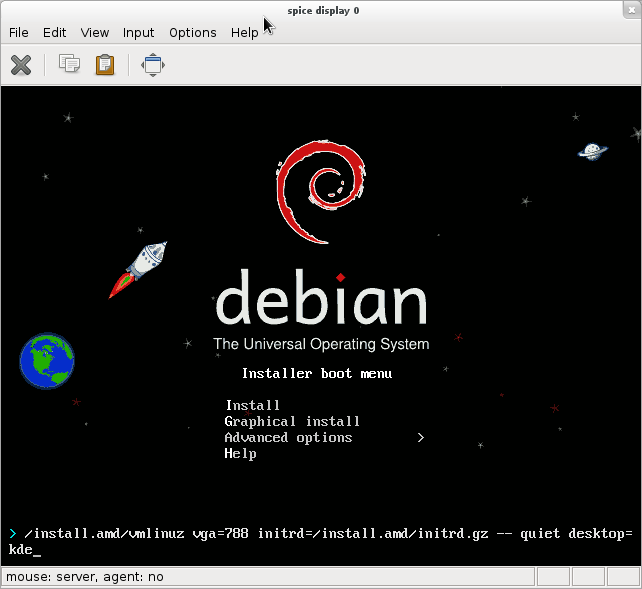
\includegraphics[width=8cm]{image201202/kdedesk/stable-inst-menu.png}
\end{center}
\end{frame}

\begin{frame}[containsverbatim]{安定版のKDE環境インストール方法3/5}
4. 画面下に出てきたエディット画面で、''desktop=kde''を追加。\\
\begin{commandline}
 /install.amd/vmlinuz vga=788 initrd=/install.amd/initrd.gz 
    --- quiet desktop=kde
\end{commandline}
5. インストールを進める\\
6. 「インストールするソフトウェアの選択:」で''Debian desktop environment''を選択。
\end{frame}

\begin{frame}{安定版のKDE環境インストール方法4/5}
インストールするソフトウェアの選択画面
\begin{center}
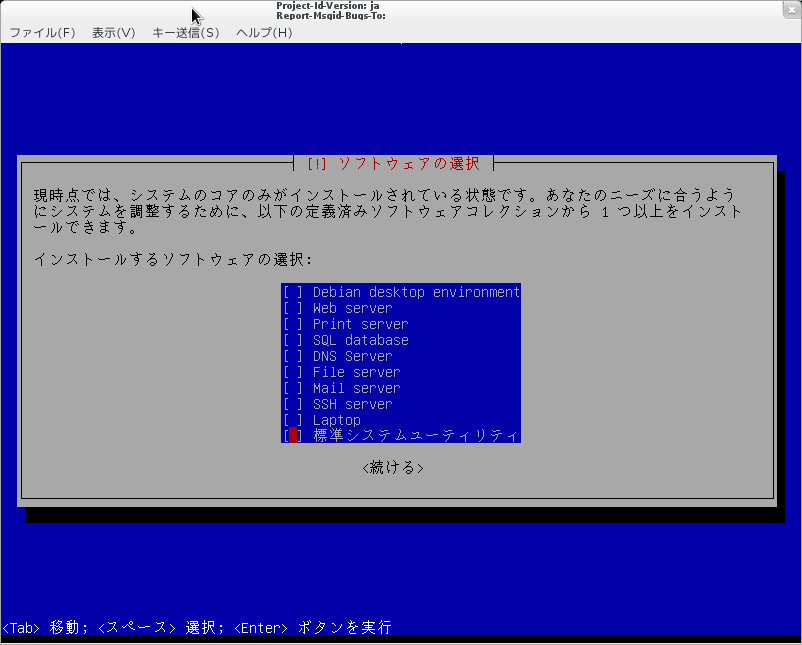
\includegraphics[width=8cm]{image201202/kdedesk/stable-inst-chooser-soft.png}
\end{center}
\end{frame}

\begin{frame}[containsverbatim]{安定版のKDE環境インストール方法5/5}
7. インストールを継続し、完了させ、リブート\\
8. グラフィカルなログインが現れる。\\

以上となります。
\end{frame}

\begin{frame}{東京エリアDebian勉強会関係者の独白}
\begin{center}
\Large
東京エリアDebian勉強会関係者談: \\
「安定版なんてぬるすぎるのだ!!」\\
「こんなのつまらない、なんてぬるげー」
\end{center}
\end{frame}

\begin{frame}{モバイルでExperimental版を持ち歩け!}
開発環境: ノートパソコンにモデム(モバイルWifiでもいいよ!)
\begin{center}
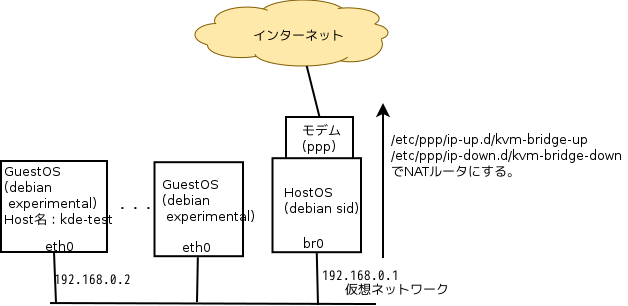
\includegraphics[width=10cm]{image201202/kdedesk/kde-dev-env.png}
\end{center}
\end{frame}

\begin{frame}{なんでKVM 1/2}
\begin{center}
{\Large
いろいろ細かい事できるから。\\
本当はVT-dも欲しかった...} \\

VT-dあればHostOSのPCIデバイスをGuestOSのPCIへほぼ直接マッピングできる気がー。リモートkernel debuggerごと動かせるんちゃうー?\\
\end{center}
※やったことないけどね...本当にできたら夢と理想の組み込み開発環境の出来上がり。素敵ー
\end{frame}

\begin{frame}{なんでKVM 2/2}
\begin{center}
{\Large
VD-Iとしてspice使いたかったのです。\\
}
\end{center}
※音もでるよ!動画もmjpeg圧縮かかるので最適、いろいろ仮想デスクトップ
向きとのとのうたい文句。\url{http://www.spice-space.org/}
\end{frame}

\begin{frame}{脱線:spiceの現実}
\begin{itemize}
\item 反応速度はVNCとあまり変わらんきが...
\item Youtubeであればコマ落ちしないというのはどうなんだろう...自分とこではコマ落ちしまくり...
\item Debian提供のものはバグる、落ちる!
\item 音も、まあ、途切れますなぁ。
\end{itemize}
但し、自分の使い方が間違っているのかも!将来に期待!(VNCよりは可能性あり)
\end{frame}

\begin{frame}{Experimenal環境導入}
詳しくは、東京エリアDebian勉強会資料をみてくださいませ。\\
導入のコツ:
\begin{enumerate}
\item 名刺サイズのCDイメージ使って、sid版を直接導入。
\item sid側でKDE導入しても、experimental版導入でsid側のKDE環境は見事上書きなので、無駄を省くため、sidは最小限インストールで。
\item task-hogeという便利なパッケージがあるので、こちらを活用。
\end{enumerate}
\end{frame}

\begin{frame}{パッケージ開発Tips}

KDEはバージョン4からautotoolsから足を洗った。

The Road to KDE 4: CMake, a New Build System for KDE\\
\url{http://dot.kde.org/2007/02/21/road-kde-4-cmake-new-build-system-kde}
\\
Why the KDE project switched to CMake -- and how (continued)\\
\url{http://lwn.net/Articles/188693/}

なので、debhelperもこちらに対応する必要あり。

\end{frame}

\begin{frame}{ありがとう!pkg-kde-tools}
DebianではKDE開発の為のツール群と、debhelper拡張用モジュールを提供しており、
パッケージ開発が容易になっている状況です。
\end{frame}

\begin{frame}[containsverbatim]{やってみようHellow worldパッケージ}
詳しいことは、東京エリアDebian勉強会資料ですが、debian/rulesだけ書いときます。
\begin{commandline}
#!/usr/bin/make -f

%:
       dh $@ --with kde
\end{commandline}
%$
ありがとう!pkg-kde-tools!僕にもできたよ!
\end{frame}

\begin{frame}[containsverbatim]{パッチあてて、本格開発}
すみません、そこまでいけてません。
きっと、
\begin{commandline}
#!/usr/bin/make -f

%:
       dh $@ --with quilt,kde

\end{commandline}
%$
かな...と思ってます。

kdeutils-4.7.4のdebian/rulesとか見てみたんですが、残念なことにv8/v9チックな書き方になっておらず、読み物としてはおもしろいのですが、参考にならず...。
\end{frame}

\begin{frame}{pkg-kde-toolsパッケージの自分的課題}
ちょっと使い出がわからないコマンド/モジュールが多数...
\begin{itemize}
\item dh\_sameversiondep
\item dh\_sodeps
\item pkgkde-ほげコマンド群\\
(pkgkde-debs2symbols,pkgkde-gensymbols,pkgkde-symbolshelper等...)
\item Debhelper/Sequence/sodeps.pmとか、lib/Dpkg/Shlibs/Objdump.pmとか、Dpkg/Shlibs/Cppfilt.pmtとか
\end{itemize}
\begin{center}
きっと、このあたりが魔窟に違いない...
\end{center}
\end{frame}

\section{月刊Debhelper 第4回}
\emtext{月刊Debhelper 第4回}

\section{cmake使ってみた}
\emtext{cmake使ってみた}

\section{今後のイベント}
\emtext{今後のイベント}
\begin{frame}{今後のイベント}
\begin{itemize}
 \item 3月 Debian勉強会 in OSC Tokyo
\end{itemize}
詳しくは\url{http://www.ospn.jp/osc2012-spring/}。お手伝い絶賛募集中!
\end{frame}

\section{今日の宴会場所}
\emtext{今日の宴会場所}

\end{document}

;;; Local Variables: ***
;;; outline-regexp: "\\([ 	]*\\\\\\(documentstyle\\|documentclass\\|emtext\\|section\\|begin{frame}\\)\\*?[ 	]*[[{]\\|[]+\\)" ***
;;; End: ***
